% !TEX program = xelatex
\documentclass[aspectratio=169,10pt]{beamer}
\usepackage{fontspec}
\usepackage{graphicx,booktabs,array,amsmath,tabularx}
\setsansfont{DejaVu Sans}
\setmonofont{DejaVu Sans Mono}
\usetheme{metropolis}
\metroset{progressbar=none}
\definecolor{navy}{HTML}{103752}
\definecolor{teal}{HTML}{148F91}
\definecolor{titlebg}{HTML}{D9E9EE}
\setbeamercolor{frametitle}{fg=navy,bg=titlebg}
\setbeamercolor{alerted text}{fg=teal}
\setbeamercolor{section header}{fg=white,bg=navy}
\setbeamerfont{section header}{size=\small}
\setbeamertemplate{headline}{%
  \leavevmode%
  \begin{beamercolorbox}[wd=\paperwidth,ht=3.2ex,dp=1.4ex,leftskip=9mm,rightskip=9mm]{section header}%
    \textbf{PHẦN \insertsectionnumber}\hspace{0.8em}\insertsectionhead
  \end{beamercolorbox}%
}
\setbeamertemplate{navigation symbols}{}
\setbeamertemplate{footline}[frame number]
\setbeamertemplate{section in toc}[sections numbered]
\setbeamersize{text margin left=9mm,text margin right=9mm}
\graphicspath{{./}{figs/}{artifacts/plots/}{evaluation/}}
\newcommand{\smallsource}[1]{\par\vspace{0.3em}{\tiny\color{gray}Nguồn: #1}}
\newcommand{\emphnum}[1]{{\color{teal}\bfseries #1}}

\title{Phân loại ảnh CIFAR-100}
\subtitle{Wide ResNet-16-4 và EfficientNetV2-B0}
\author{Đinh Quang Bách, Đinh Hồng Hiệp, Nguyễn Văn Huy Hiệu}
\date{Tháng 10 năm 2026}

\begin{document}

\begin{frame}[plain]{}
  \begin{center}
    \vspace{0.5em}
    {\LARGE\bfseries\color{navy}PHÂN LOẠI ẢNH CIFAR-100\par}
    \vspace{0.6em}
    {\large Wide ResNet-16-4 và EfficientNetV2-B0\par}
    \vspace{1.4em}
    {\normalsize\bfseries Nhóm:\par}
    \vspace{0.3em}
    {\normalsize Đinh Quang Bách\par}
    {\normalsize Đinh Hồng Hiệp\par}
    {\normalsize Nguyễn Văn Huy Hiệu\par}
    \vspace{1.2em}
    {\small Tháng 10 năm 2026\par}
  \end{center}
\end{frame}

\begin{frame}[plain]{}
  {\Large\bfseries\color{navy}Mục lục\par}
  \vspace{0.8em}
  \large
  \begin{enumerate}
    \setlength{\itemsep}{0.55em}
    \item Bài toán và thiết kế thực nghiệm
    \item Hai mô hình và cách huấn luyện
    \item Kết quả thực nghiệm
    \item Diễn giải và kết luận
    \item Phụ lục
  \end{enumerate}
\end{frame}

\section{Bài toán và thiết kế thực nghiệm}

\begin{frame}{Bài toán và câu hỏi thực nghiệm}
  \begin{itemize}
    \item Phân loại ảnh RGB $32\times32$ vào một trong \textbf{100 lớp} của CIFAR-100.
    \item So sánh \textbf{WRN-16-4 huấn luyện từ đầu} với \textbf{EfficientNetV2-B0 fine-tune từ mô hình đã học trên ImageNet}.
    \item Đánh giá trên tập test bằng Top-1, macro-F1 và kết quả theo từng lớp.
  \end{itemize}
  \vspace{0.7em}
  \begin{block}{Câu hỏi chính}
    Trên cùng tập test, hai mô hình đạt kết quả ra sao? Những khác biệt trong cách huấn luyện ảnh hưởng thế nào đến việc so sánh?
  \end{block}
\end{frame}

\begin{frame}{CIFAR-100 và cách chia dữ liệu}
  \begin{columns}[T,onlytextwidth]
    \column{.50\textwidth}
    \begin{itemize}
      \item \textbf{60.000} ảnh màu $32\times32$ thuộc \textbf{100 lớp}.
      \item Tập train gốc có \textbf{50.000} ảnh; tập test có \textbf{10.000} ảnh.
      \item Chia tập train gốc thành \textbf{45.000 ảnh train} và \textbf{5.000 ảnh validation}.
      \item Chỉ đánh giá trên test sau khi đã chọn checkpoint.
    \end{itemize}
    \column{.46\textwidth}
    \begin{tabular}{lr}
      \toprule
      Vai trò & Số ảnh \\
      \midrule
      Huấn luyện & 45.000 \\
      Chọn checkpoint & 5.000 \\
      Đánh giá cuối & 10.000 \\
      \bottomrule
    \end{tabular}
  \end{columns}
  \vspace{0.8em}
  \begin{alertblock}{Cách tạo tập validation}
    Hai notebook hiện dùng cùng phép hoán vị NumPy (seed 42) và lấy 5.000 ảnh đầu làm validation. Kết quả EfficientNet đã lưu thuộc lần chạy trước khi thống nhất cách chia này.
  \end{alertblock}
  \smallsource{build\_wrn.ipynb; build\_efficientnet.ipynb, cell chia dữ liệu.}
\end{frame}

\begin{frame}{Quy trình thực nghiệm chung}
  \small
  \begin{tabularx}{\linewidth}{@{}p{.20\linewidth}X@{}}
    \toprule
    Bước & Cách thực hiện \\
    \midrule
    Chia dữ liệu & 50.000 ảnh train gốc $\rightarrow$ 45.000 train + 5.000 validation; giữ riêng 10.000 test. \\
    Augmentation theo ảnh & Lật ngang 50\%; reflection padding 4 px + crop $32\times32$; color jitter 80\%; Cutout 25\% / Random Erasing 25\% / không che ảnh 50\%. \\
    Chuẩn bị đầu vào & WRN: $32\times32$, chuẩn hóa theo tập train. EfficientNet: $224\times224$, chuẩn hóa ImageNet. \\
    Augmentation theo batch & MixUp 30\%, CutMix 30\% hoặc không trộn 40\%. \\
    Validation và test & Không áp dụng augmentation ngẫu nhiên; dùng bước chuẩn bị đầu vào của từng mô hình. \\
    Chọn checkpoint & Lấy checkpoint có \texttt{val\_loss} thấp nhất, rồi đánh giá trên test. \\
    \bottomrule
  \end{tabularx}
  \vspace{0.5em}
  \begin{block}{Các bước dùng chung và bước riêng}
    Augmentation giống nhau; kích thước ảnh và cách chuẩn hóa tùy theo backbone.
  \end{block}
\end{frame}

\begin{frame}{Augmentation dùng cho cả hai mô hình}
  \begin{columns}[T,onlytextwidth]
    \column{.48\textwidth}
    \textbf{Với từng ảnh train $32\times32$}
    \begin{enumerate}
      \item Lật ngang ngẫu nhiên ($p=0{,}5$).
      \item Reflection padding 4 pixel, rồi crop về $32\times32$.
      \item Color jitter nhẹ ($p=0{,}8$).
      \item Chọn \textbf{một cách xử lý}: Cutout 25\%, Random Erasing 25\%, không che ảnh 50\%.
    \end{enumerate}
    \column{.48\textwidth}
    \textbf{Với từng batch train}
    \begin{itemize}
      \item MixUp 30\%, $\alpha=0{,}5$.
      \item CutMix 30\%, $\alpha=1$.
      \item Không trộn 40\%.
      \item Ảnh và nhãn được trộn theo cùng tỷ lệ; với CutMix, tỷ lệ nhãn dựa trên diện tích vùng được thay thế.
    \end{itemize}
  \end{columns}
  \vspace{0.25em}
  \begin{alertblock}{Validation và test}
    Không áp dụng augmentation ngẫu nhiên. Notebook EfficientNet đã được cập nhật theo chính sách này, nhưng cần chạy lại để có kết quả tương ứng.
  \end{alertblock}
  \smallsource{build\_wrn.ipynb, các cell augmentation; build\_efficientnet.ipynb, các cell 4 và 9.}
\end{frame}

\begin{frame}{Augmentation theo ảnh: trước và sau}
  \centering
  \includegraphics[width=.95\linewidth,height=.55\textheight,keepaspectratio]{wrn_before_after_augmentation.png}
  \vspace{0.2em}
  \\
  {\small Lật ngang $\rightarrow$ reflection crop $\rightarrow$ color jitter $\rightarrow$ Cutout / Random Erasing / không che ảnh.}
  \vspace{0.15em}
  \\
  {\scriptsize Mỗi cột là cùng một ảnh; kết quả thay đổi theo lựa chọn ngẫu nhiên ở từng bước.}
  \smallsource{artifacts/plots/wrn\_before\_after\_augmentation.png.}
\end{frame}

\begin{frame}{Augmentation theo batch: MixUp và CutMix}
  \centering
  \includegraphics[width=.98\linewidth,height=.58\textheight,keepaspectratio]{wrn_mixup_cutmix_preview.png}
  \vspace{0.35em}
  \\
  {\small Sau augmentation theo ảnh, MixUp hòa trộn toàn ảnh; CutMix thay một vùng ảnh. Cả hai cũng trộn nhãn.}
  \vspace{0.2em}
  \\
  {\scriptsize Hình dùng tỷ lệ cố định để dễ quan sát; khi train, tỷ lệ trộn và vị trí vùng thay thế được chọn ngẫu nhiên.}
  \smallsource{artifacts/plots/wrn\_mixup\_cutmix\_preview.png.}
\end{frame}

\section{Hai mô hình và cách huấn luyện}

\begin{frame}{Hai cách tiếp cận}
  \begin{tabularx}{\linewidth}{@{}p{.28\linewidth}XX@{}}
    \toprule
    & Wide ResNet-16-4 & EfficientNetV2-B0 \\
    \midrule
    Khởi tạo & Trọng số ngẫu nhiên & Trọng số pretrained trên ImageNet \\
    Kích thước đầu vào & $32\times32$ & $224\times224$ sau resize \\
    Thành phần chính & Residual blocks và shortcut & Fused-MBConv / MBConv \\
    Lớp phân loại & Global average pooling $\rightarrow$ Dense(100) & Global pooling $\rightarrow$ classifier 100 lớp \\
    Framework & TensorFlow/Keras & PyTorch/timm \\
    \bottomrule
  \end{tabularx}
  \vspace{0.8em}
  \begin{block}{Điểm chung}
    Hai mô hình giải cùng bài toán, dùng cùng tập test và quy trình augmentation. Cách khởi tạo và kích thước đầu vào khác nhau.
  \end{block}
\end{frame}

\begin{frame}{Residual block trong WRN}
  \begin{columns}[T,onlytextwidth]
    \column{.48\textwidth}
    \begin{block}{Nhánh chính}
      BN $\rightarrow$ ReLU $\rightarrow$ Conv $3\times3$ $\rightarrow$ BN $\rightarrow$ ReLU $\rightarrow$ Conv $3\times3$.
    \end{block}
    \column{.48\textwidth}
    \begin{block}{Shortcut}
      Giữ nguyên $x$ khi kích thước khớp; dùng Conv $1\times1$ khi cần đổi số kênh hoặc giảm kích thước feature map.
    \end{block}
  \end{columns}
  \vspace{0.5em}
  \[y=F(x)+S(x)\]
  \begin{itemize}
    \item Đầu ra của block là tổng của nhánh chính và nhánh shortcut.
    \item WRN-16-4 có hai residual blocks trong mỗi nhóm; hệ số mở rộng kênh là 4.
  \end{itemize}
  \smallsource{src/cifar\_classifier/model.py.}
\end{frame}

\begin{frame}{Wide ResNet-16-4: kiến trúc tổng thể}
  \begin{columns}[T,onlytextwidth]
    \column{.23\textwidth}
    \footnotesize\raggedright
    \begin{itemize}
      \item Conv $3\times3$ đầu tiên: 16 kênh.
      \item Ba nhóm residual: 64, 128, 256 kênh.
      \item Hai blocks mỗi nhóm.
      \item Downsample ở nhóm 2 và 3.
      \item Global pooling $\rightarrow$ Dense(100).
    \end{itemize}
    \column{.74\textwidth}
    \centering
    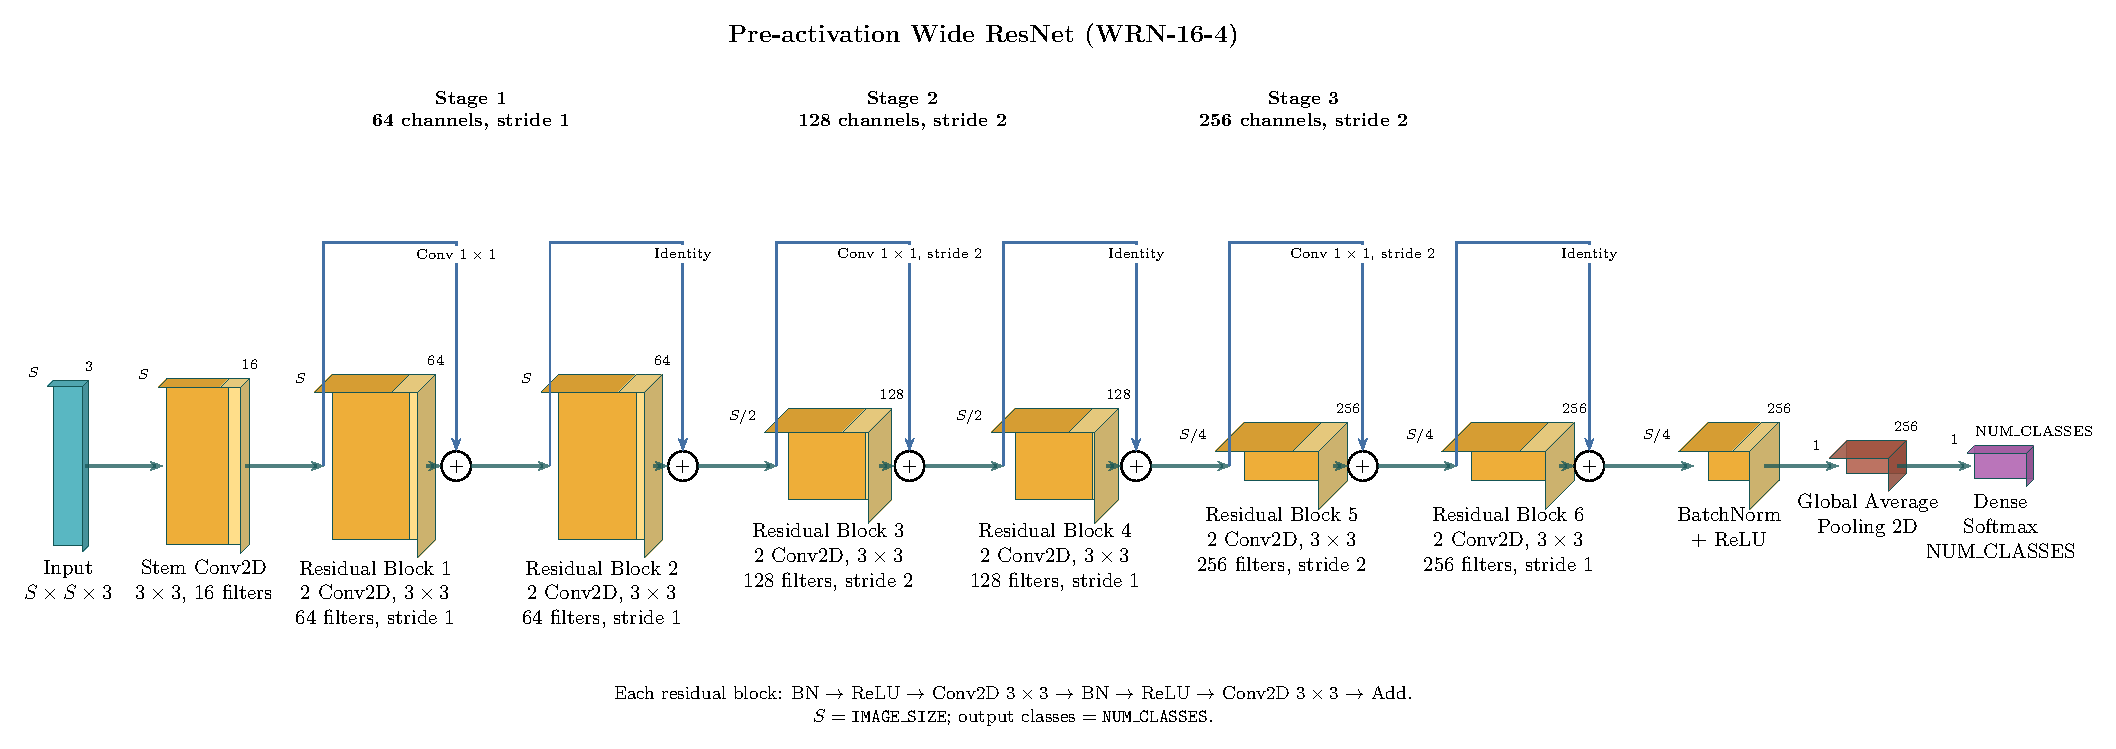
\includegraphics[width=\linewidth,height=.82\textheight,keepaspectratio]{wide_resnet_architecture.pdf}
  \end{columns}
  \smallsource{src/cifar\_classifier/model.py; wide\_resnet\_architecture.pdf.}
\end{frame}

\begin{frame}{EfficientNetV2-B0: kiến trúc và đầu vào}
  \begin{itemize}
    \item Dùng backbone \texttt{tf\_efficientnetv2\_b0.in1k} trong \texttt{timm}, với trọng số pretrained trên ImageNet.
    \item Thay classifier cuối bằng đầu ra \textbf{100 lớp}; đặt dropout \textbf{0,3} và fine-tune toàn bộ mô hình.
    \item Áp dụng augmentation khi ảnh còn ở $32\times32$, rồi resize lên $224\times224$.
    \item Dùng mean/std ImageNet để chuẩn hóa đầu vào cho backbone pretrained.
  \end{itemize}
  \smallsource{build\_efficientnet.ipynb, cells khởi tạo mô hình và transforms.}
\end{frame}

\begin{frame}{Cấu hình huấn luyện và chọn checkpoint}
  \small
  \begin{tabularx}{\linewidth}{@{}p{.29\linewidth}XX@{}}
    \toprule
    Thành phần & WRN-16-4 & EfficientNetV2-B0 \\
    \midrule
    Batch size & 64 & 32 \\
    Optimizer & AdamW, LR $10^{-3}$ & AdamW, LR $2\times10^{-5}$ \\
    Weight decay & $10^{-4}$ & $10^{-4}$ \\
    Hàm loss & Categorical cross-entropy & Cross-entropy, label smoothing 0,1 \\
    Scheduler & ReduceLROnPlateau & ReduceLROnPlateau \\
    Số epoch tối đa & 200 & 30 \\
    Early stopping & Patience 20 & Patience 4 \\
    Chọn checkpoint & Validation loss thấp nhất & Validation loss thấp nhất \\
    \bottomrule
  \end{tabularx}
  \smallsource{src/cifar\_classifier/train.py; build\_efficientnet.ipynb, cells 2, 7, 9.}
\end{frame}

\begin{frame}{Chỉ số đánh giá}
  \begin{itemize}
    \item \textbf{Top-1}: tỷ lệ ảnh mà lớp có xác suất cao nhất trùng với nhãn thật.
    \item \textbf{Macro-F1}: trung bình F1 của 100 lớp, mỗi lớp có trọng số ngang nhau.
    \item \textbf{Confusion matrix}: cho thấy số ảnh của mỗi lớp bị nhầm sang các lớp khác.
  \end{itemize}
  \vspace{0.5em}
  \begin{block}{Nguyên tắc đánh giá}
    Chọn checkpoint có validation loss thấp nhất, nạp lại checkpoint đó và đánh giá trên 10.000 ảnh test. Tập test không tham gia chọn checkpoint.
  \end{block}
\end{frame}

\section{Kết quả thực nghiệm}

\begin{frame}{WRN: kết quả huấn luyện qua 94 epoch}
  \centering
  \includegraphics[width=.95\linewidth,height=.69\textheight,keepaspectratio]{cifar100_wrn16_4_aug200_history.png}
  \vspace{0.2em}
  \\
  {\small Validation loss thấp nhất ($\approx0{,}9590$) và validation accuracy cao nhất ($\approx74{,}48\%$) cùng ở epoch 74.}
  \smallsource{checkpoints/cifar100\_wrn16\_4\_aug200\_history.csv; artifacts/plots/cifar100\_wrn16\_4\_aug200\_history.png.}
\end{frame}

\begin{frame}{EfficientNet: kết quả huấn luyện đã lưu}
  \centering
  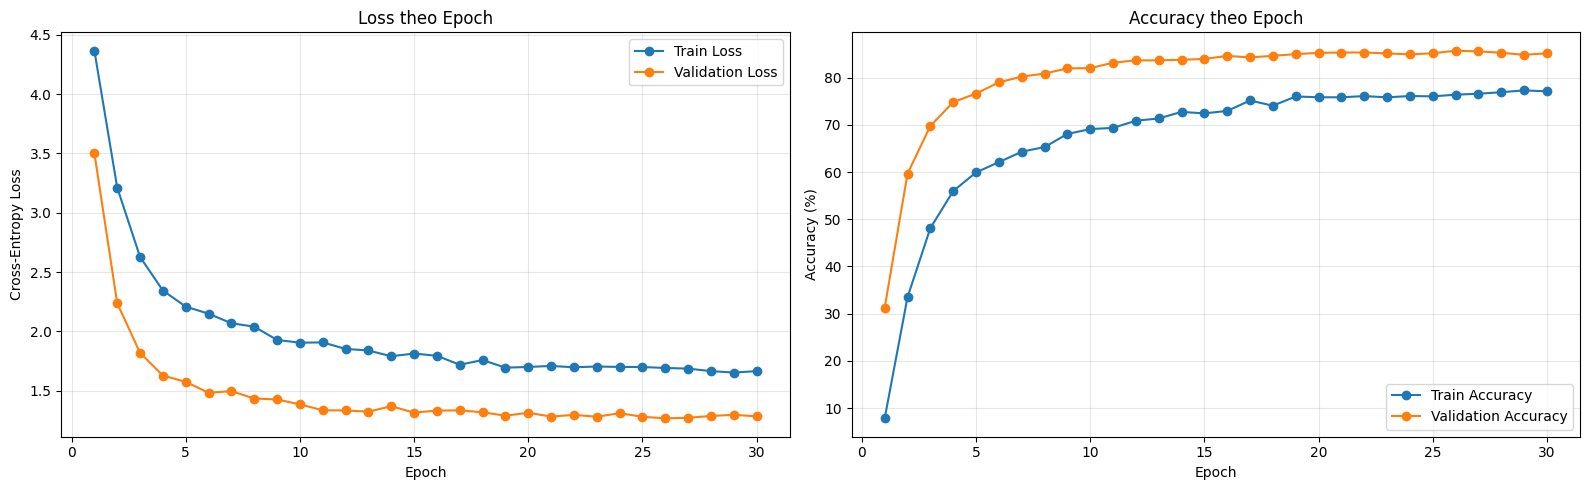
\includegraphics[width=.95\linewidth,height=.67\textheight,keepaspectratio]{efficient_training_previous.png}
  \vspace{0.2em}
  \\
  {\small Chạy đủ 30 epoch; validation loss thấp nhất ở epoch 26 ($1{,}2671$).}
  \smallsource{Biểu đồ từ output build\_efficientnet.ipynb. Lần chạy này có trước khi thống nhất hoàn toàn augmentation và cách chia tập.}
\end{frame}

\begin{frame}{Kết quả trên tập test}
  \begin{tabularx}{\linewidth}{@{}p{.36\linewidth}XX@{}}
    \toprule
    Chỉ số & WRN-16-4 & EfficientNetV2-B0 \\
    \midrule
    Epoch đã chạy / checkpoint & 94 / 74 & 30 / 26 \\
    Top-1 test & \emphnum{74,05\%} & \emphnum{84,95\%} \\
    Macro-F1 & 73,97\% & Xấp xỉ 84,9\% \\
    Chênh lệch Top-1 & \multicolumn{2}{c}{EfficientNet cao hơn \textbf{10,90 điểm phần trăm}} \\
    \bottomrule
  \end{tabularx}
  \vspace{0.6em}
  \begin{alertblock}{Lưu ý về kết quả}
    Số liệu EfficientNet thuộc lần chạy trước khi hoàn tất việc đồng bộ với WRN. Cần chạy lại EfficientNet để có kết quả theo quy trình hiện tại.
  \end{alertblock}
  \smallsource{evaluation/wrn\_test\_metrics.json; output đánh giá và classification report trong build\_efficientnet.ipynb.}
\end{frame}

\begin{frame}{WRN: các cặp lớp thường bị nhầm}
  \small
  \begin{tabular}{@{}llr@{}}
    \toprule
    Nhãn thật & Dự đoán thành & Số ảnh bị nhầm \\
    \midrule
    maple\_tree & oak\_tree & 21 \\
    girl & woman & 19 \\
    woman & girl & 19 \\
    man & boy & 18 \\
    willow\_tree & maple\_tree & 16 \\
    \bottomrule
  \end{tabular}
  \vspace{0.5em}
  \begin{itemize}
    \item Những lỗi nổi bật nằm ở các cặp lớp tương tự nhau, chẳng hạn các loại cây hoặc nhóm người.
    \item Các lớp có F1 thấp nhất: otter 42,27\%, girl 45,90\%, shrew 46,31\%, seal 47,29\%, boy 50,25\%.
  \end{itemize}
  \smallsource{evaluation/wrn\_confusion\_matrix.csv; evaluation/wrn\_classification\_report.csv.}
\end{frame}

\section{Diễn giải và kết luận}

\begin{frame}{Giới hạn khi so sánh hai mô hình}
  \begin{itemize}
    \item Trong hai lần chạy đã lưu, EfficientNetV2-B0 cao hơn WRN-16-4 \textbf{10,90 điểm phần trăm Top-1}.
    \item EfficientNet dùng trọng số \textbf{pretrained trên ImageNet}; WRN được huấn luyện từ đầu.
    \item Hai mô hình còn khác kích thước đầu vào, hàm loss, batch size và lịch huấn luyện.
    \item Hai notebook hiện dùng cùng quy trình augmentation và cách chia train/validation, nhưng số liệu cũ chưa phản ánh các thay đổi này.
  \end{itemize}
  \begin{block}{Có thể kết luận gì?}
    Chênh lệch 10,90 điểm phần trăm là kết quả của \textbf{hai cách huấn luyện đang được báo cáo}; chưa thể quy riêng chênh lệch này cho kiến trúc.
  \end{block}
\end{frame}

\begin{frame}{Kết luận và bước tiếp theo}
  \begin{enumerate}
    \item Trên tập test, WRN-16-4 đạt \textbf{74,05\% Top-1} và \textbf{73,97\% macro-F1}.
    \item Lần chạy EfficientNet đã lưu đạt \textbf{84,95\% Top-1}; checkpoint tốt nhất ở epoch 26.
    \item Hai notebook hiện dùng cùng quy trình augmentation và cùng tập train/validation. \textbf{Bước tiếp theo: chạy lại EfficientNet} và cập nhật kết quả đánh giá.
  \end{enumerate}
\end{frame}

\begin{frame}
  \centering\vfill
  {\Huge\color{navy}\bfseries Cảm ơn!}\\[1em]
  {\large Q\&A}
  \vfill
\end{frame}

\appendix
\section{Phụ lục}

\begin{frame}{Phụ lục: confusion matrix WRN-16-4}
  \centering
  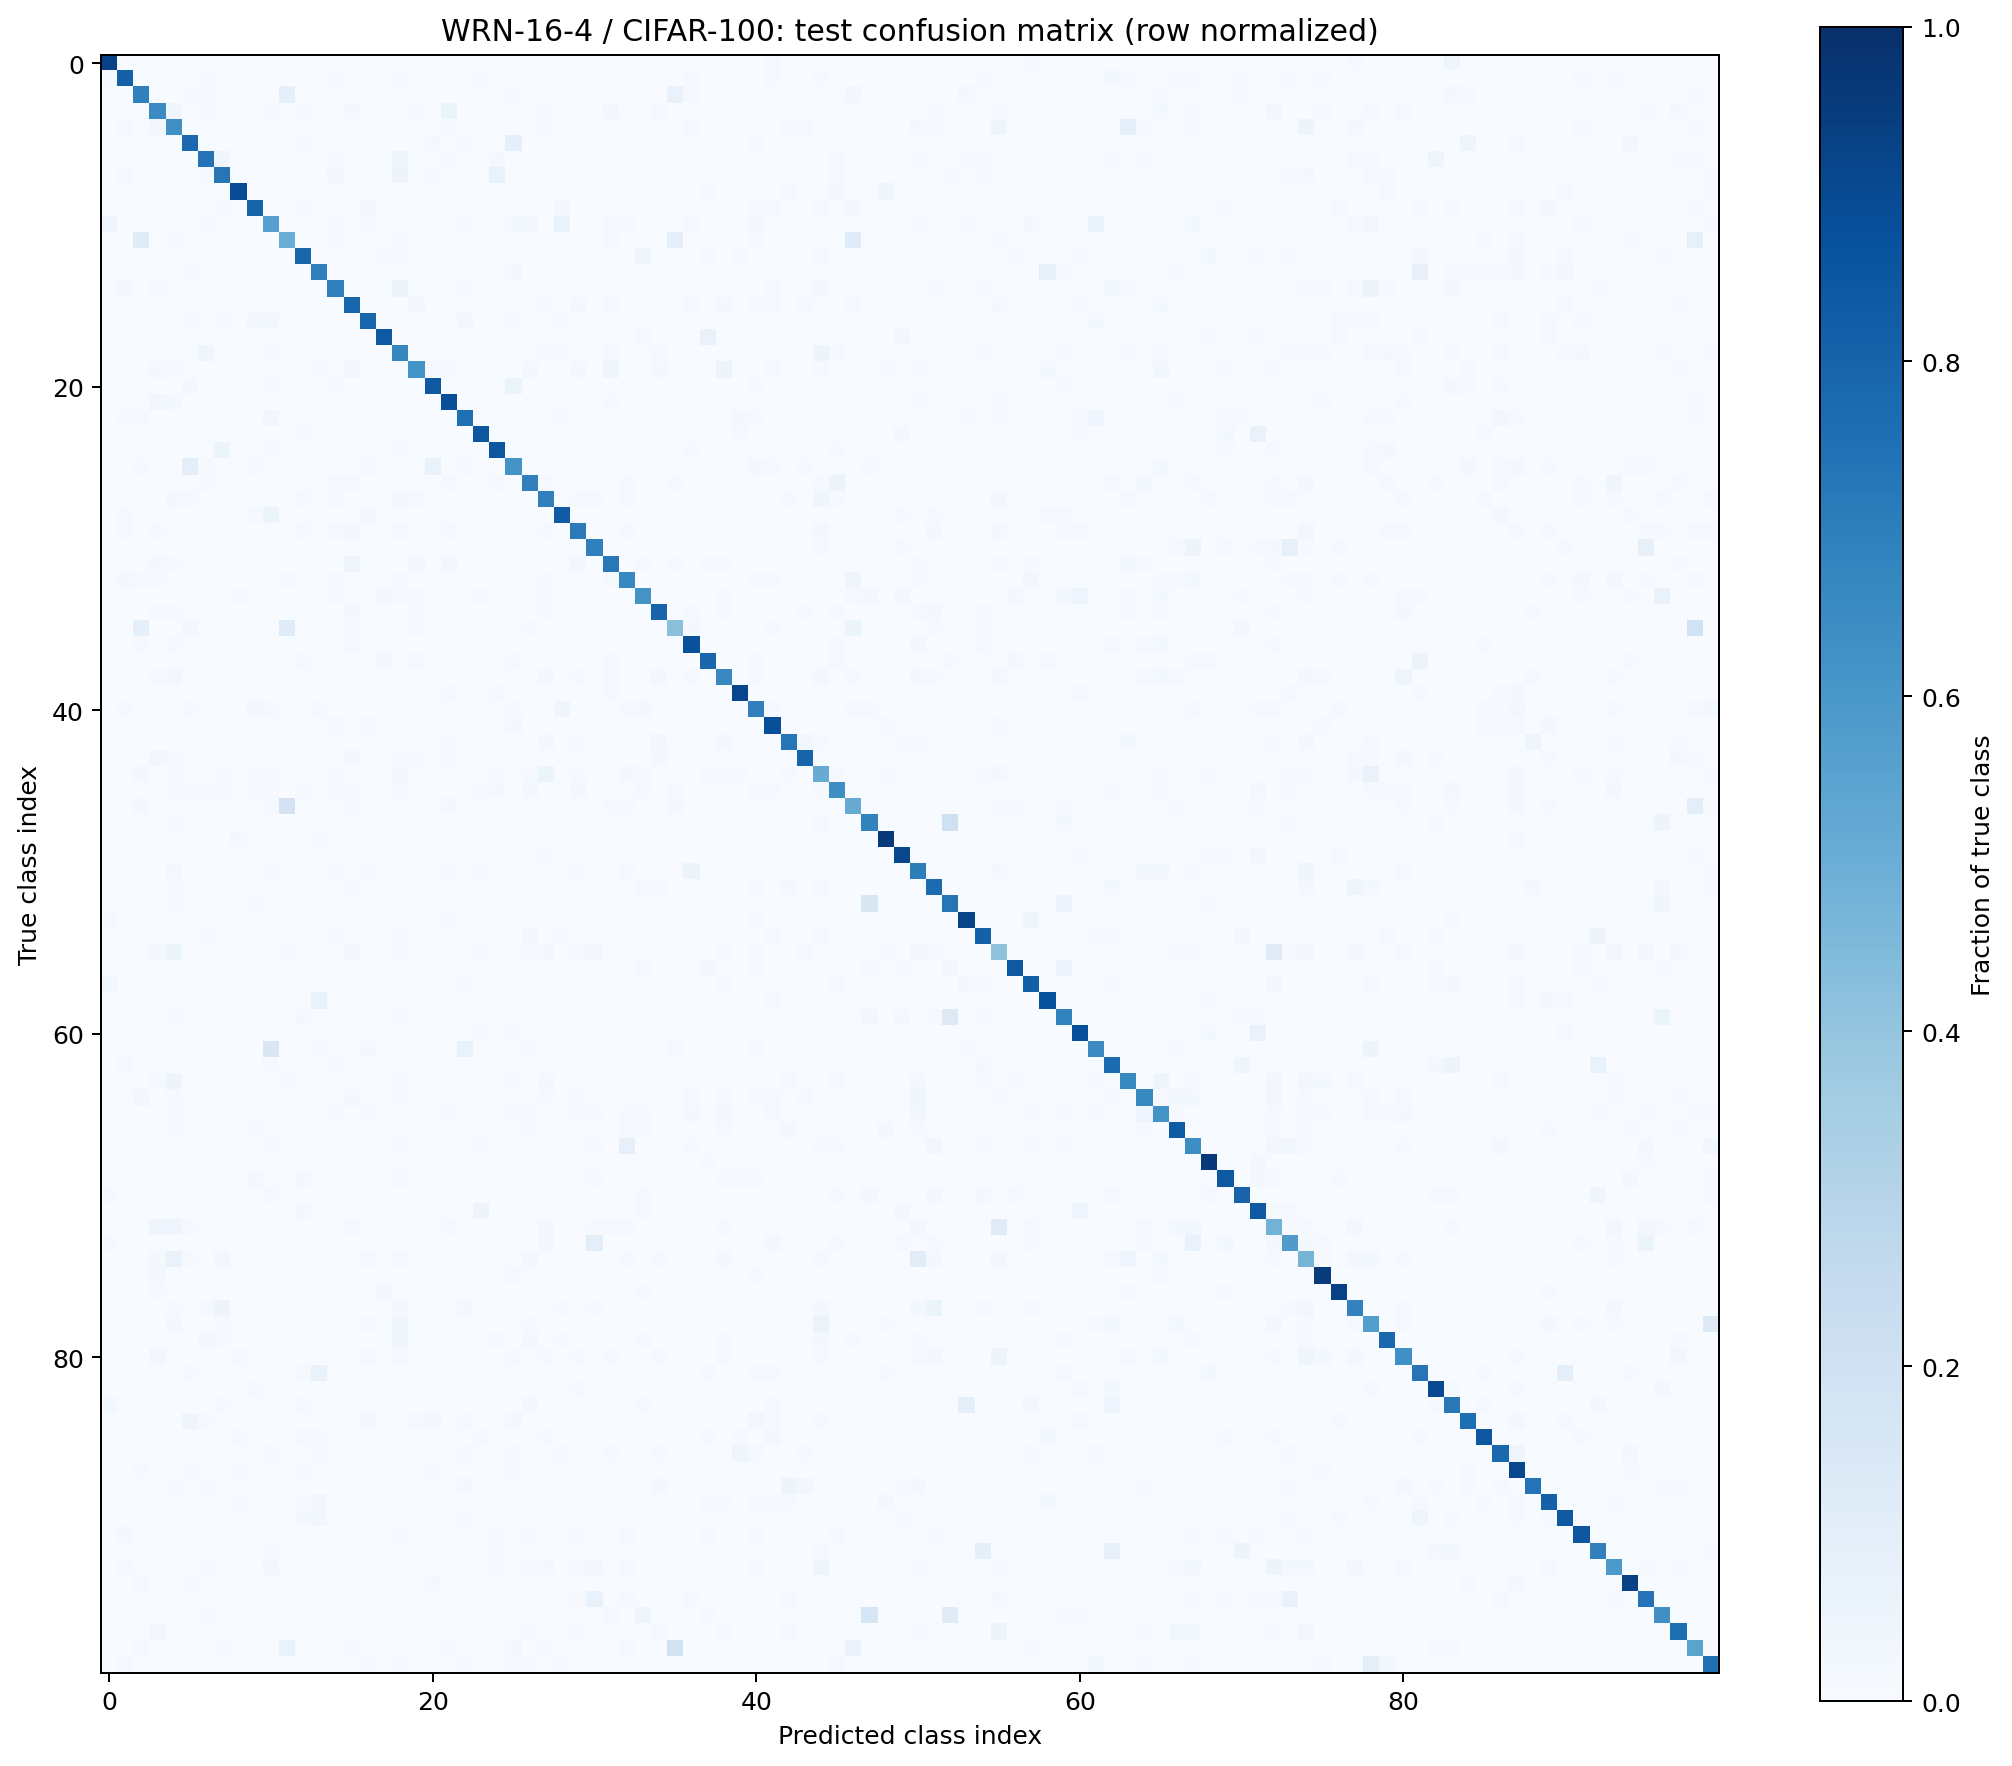
\includegraphics[width=.90\linewidth,height=.75\textheight,keepaspectratio]{wrn_confusion_matrix.png}
  \smallsource{evaluation/wrn\_confusion\_matrix.png; 10.000 ảnh test.}
\end{frame}

\begin{frame}{Phụ lục: confusion matrix EfficientNet}
  \centering
  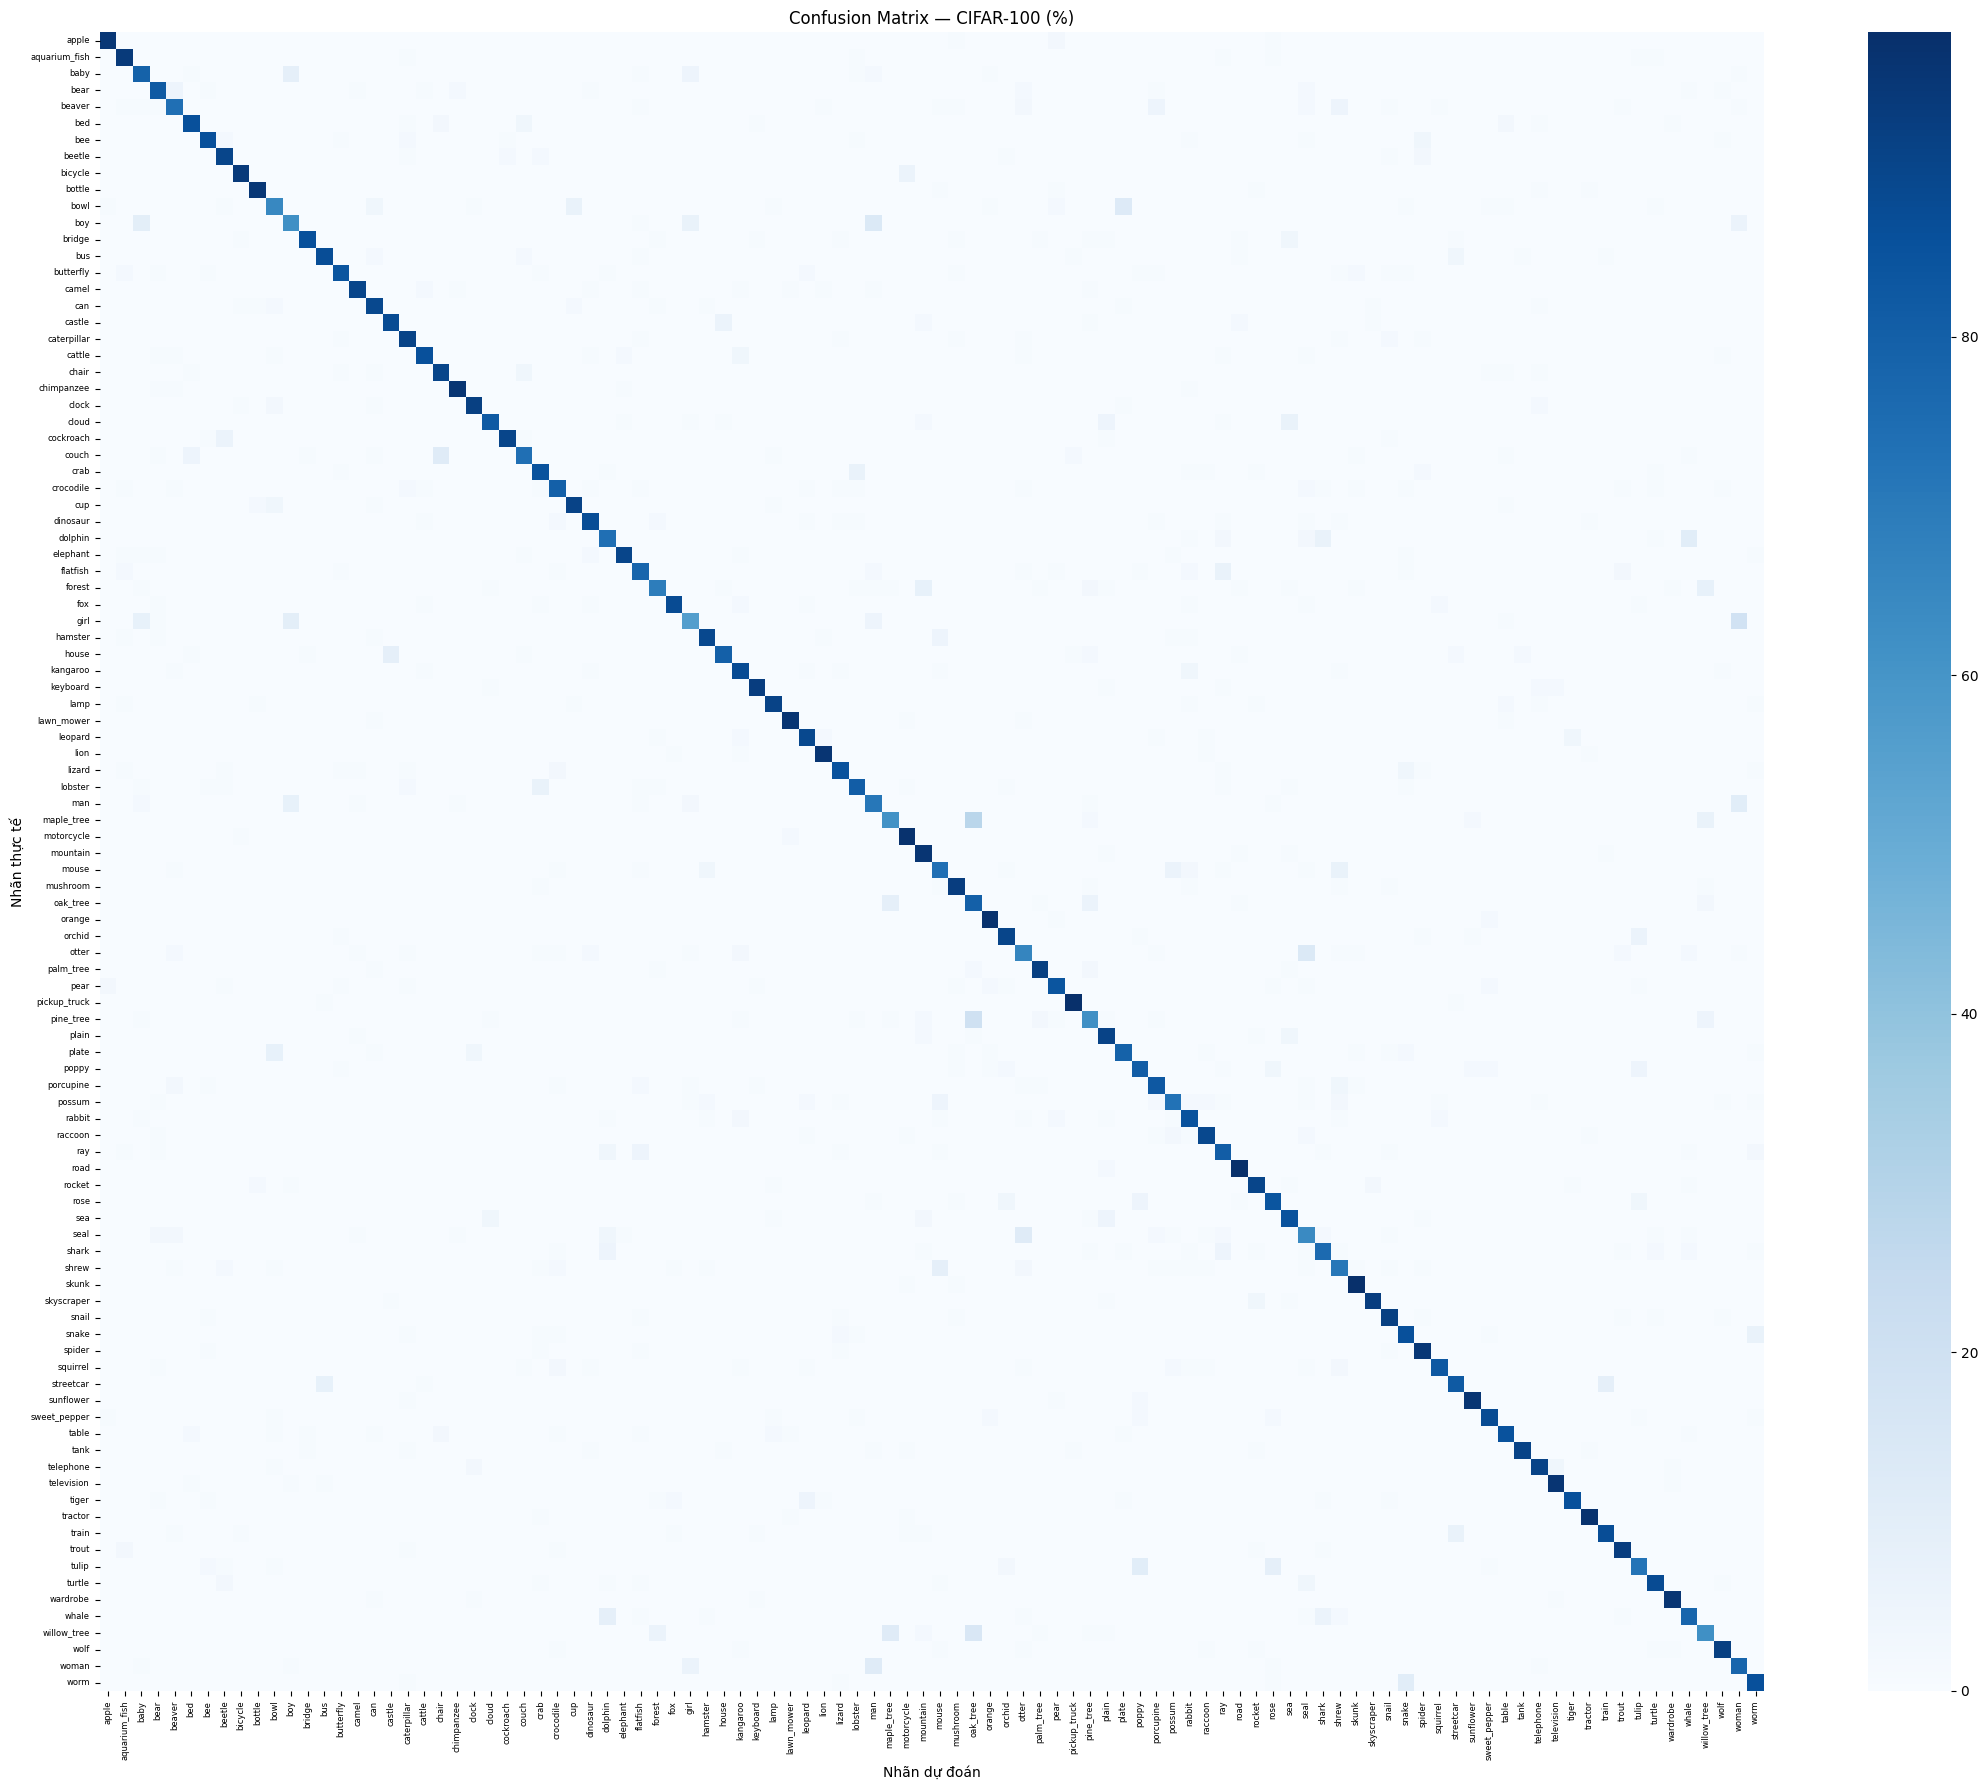
\includegraphics[width=.88\linewidth,height=.75\textheight,keepaspectratio]{efficient_confusion_previous.png}
  \smallsource{Output build\_efficientnet.ipynb, lần chạy trước khi thống nhất hoàn toàn augmentation và cách chia tập.}
\end{frame}

\end{document}
